\chapter{Fixes}

In phase 4, Team 13 performed White-box testing of our application. In their findings, they mentioned four issues to be fixed. They are as stated below.

\begin{itemize}
\item \textbf{Business Logic Data Validation} - We do not consider this as an issue, as the current implementation is similar to the real-world working. In real working, the account name does not matter and does not  have to match the account number used at the time of transaction. The only relevant factor is the \textit{Account Number} of the recipient. 
If the transfers were performed through the addition of beneficiaries, then the concept of \textit{Recipient Name} would make more sense. However, since we do not have this implementation, this could be termed as an improvement for the future.

\item \textbf{Weak SSL/TLS Ciphers} - This issue is due to the outdated software in the Virtual Machine and we opted to leave it as it is. 

\item \textbf{Error Codes} - Similar to the Weak SSL/TLS Ciphers, this is also caused due to the outdated software and we chose not to update the software for now.

\item \textbf{Guessable User Account} - This was a minor issue, where-in different error messages were displayed to the user upon failed login. The error message is now made consistent to show \enquote{Either the e-mail or the password is wrong}. So it is not possible to guess whether the account does not exist or the password is wrong.

The code change for this fix happened to just be modification of the message, as can be seen in the figure \ref{fig:fix_guessable_account}.

\end{itemize}

\begin{figure}[ht]
	\centering
	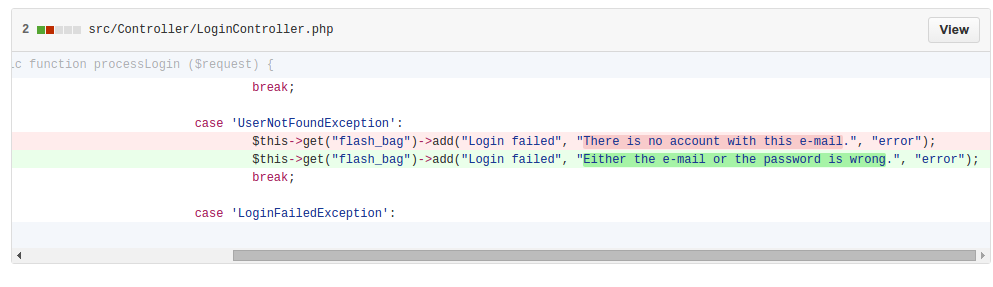
\includegraphics[width=.8\linewidth]{figures/fix_guessable_account.png}
	\caption{Code change to fix Guessable User Account}
	\label{fig:fix_guessable_account}
\end{figure}

\clearpage